


\begin{figure}[ht]
  \centering
  \begin{subfigure}[b]{0.45\linewidth}
    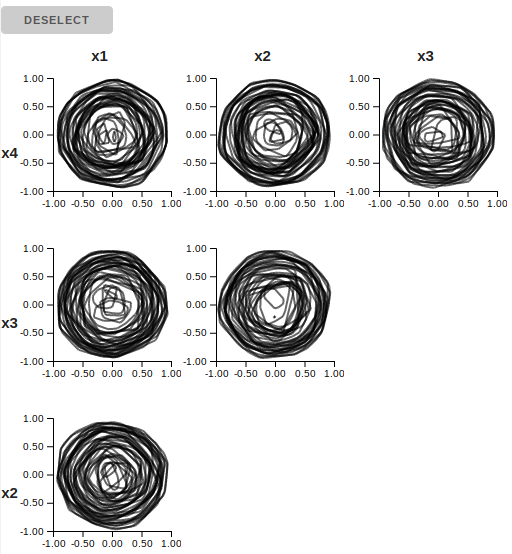
\includegraphics[width=\textwidth]{hsp_interface-global.png}
    \caption{Global view}
    \label{fig:interface:global} 
  \end{subfigure} 
  ~
  \begin{subfigure}[b]{0.45\linewidth}
    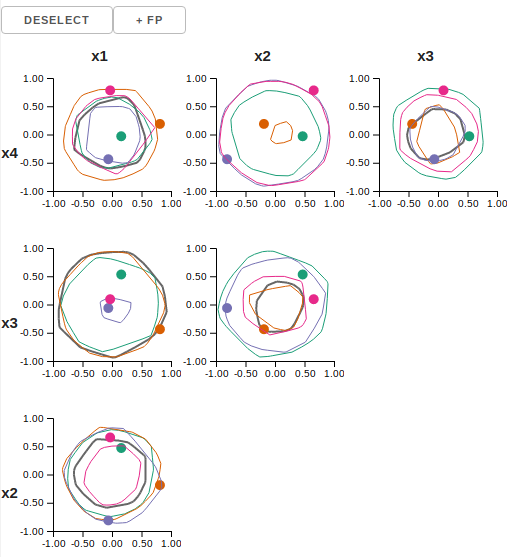
\includegraphics[width=\textwidth]{hsp_interface-local.png}
    \caption{Local view}
    \label{fig:interface:local} 
  \end{subfigure}
  \caption[The interface for browsing slices created by the Hypersliceplorer algorithm.]{%
    The interface for browsing slices created by the Hypersliceplorer algorithm.
    We show a plot for each pair of dimensions laid out in the same way as
    HyperSlice~\cite{Wijk:1993}.
    The interface has two modes: global and local view.
    The global view (\subref{fig:interface:global}) 
    shows the results of sampling over a number of focus points. The views
    are linked through highlighting a slice. The local view 
    (\subref{fig:interface:local}) shows a single selected slice and then
    the user can add additional slices by clicking the ``+ fp'' button.
  }
  \label{fig:interface}
\end{figure}

Here, I take the idea of more global overviews and revisit 2D slices
for closed multi-dimensional objects, whose overall multi-dimensional shape is
of great importance. This has been motivated by a number of real-world
application scenarios, from comprehension of multi-dimensional polytopes
(generalization of polygons to multiple dimensions) by geometers, to
applications in computational science, to multi-dimensional Pareto-front
analysis. Showing only slices of the outlines of these polytopes creates
global views of these data sets through over-plotting of many
focus points.

We address the issue of selecting a focus point by sampling a number of focus
points and producing projections of 2D slices (\autoref{fig:interface}). This
\emph{global view} gives the user an overview of the shape of the object
without having to navigate manually. Since we are viewing just
the outer hull of the object, we can draw these as a projection of a set of 2D
slices.  Linked highlighting is used to show all slices for a particular focus
point.  In addition, the user can click on a particular slice and switch to the
\emph{local view}. The local view begins by showing the particular slice the
user clicked on. The user can add additional focus points and select particular
slices for comparison. This interaction models Shneiderman's mantra: ``overview
first, filter and zoom, details on demand''~\cite{Shneiderman:1996}.

My major contribution is an
algorithm called Hypersliceplorer for computing the intersection of a 2D slice with a simplical
mesh in any dimension. The issue is that a 2D plane does not have a
well-defined normal in spaces higher than three. Therefore, one cannot
use the typical point-normal form of a plane in order to compute the
intersection of the plane with the simplex. Instead, one must treat the plane
as a point with two free parameters representing the plane. Then, 
this representation allows one to compute how a
multi-dimensional simplex intersects a 2D plane. This approach lets one compute
slices of a multi-dimensional object without a parametric form of the
surface. I also developed an interactive interface to demonstrate the results 
of this algorithm.

The algorithm and interface are evaluated in two ways representing their recommended
evaluation methods according to the nested
model~\cite{Munzner:2009}. For the overall technique and
interactive viewer, I demonstrate the effectiveness of the technique by
presenting three case studies. For the underlying algorithm I present an
analysis of the running time. 

